% Aberdeen style guide should be followed when using this
% layout. Their template powerpoint slide is used to extract the
% Aberdeen color and logo but is otherwise ignored (it has little or
% no formatting in it anyway).
%
% http://www.abdn.ac.uk/documents/style-guide.pdf

%%%%%%%%%%%%%%%%%%%% Document Class Settings %%%%%%%%%%%%%%%%%%%%%%%%%
% Pick if you want slides, or draft slides (no animations)
%%%%%%%%%%%%%%%%%%%%%%%%%%%%%%%%%%%%%%%%%%%%%%%%%%%%%%%%%%%%%%%%%%%%%%
%Normal document mode%
%\documentclass[10pt,compress,unknownkeysallowed]{beamer}
%Draft or handout mode
\documentclass[10pt,compress,handout,unknownkeysallowed]{beamer}
%\documentclass[10pt,compress,handout,ignorenonframetext,unknownkeysallowed]{beamer}

%%%%%%%%%%%%%%%%%%%% General Document settings %%%%%%%%%%%%%%%%%%%%%%%
% These settings must be set for each presentation
%%%%%%%%%%%%%%%%%%%%%%%%%%%%%%%%%%%%%%%%%%%%%%%%%%%%%%%%%%%%%%%%%%%%%%
\newcommand{\shortname}{jefferson.gomes@abdn.ac.uk}
\newcommand{\fullname}{Dr Jeff Gomes}
\institute{School of Engineering}
\newcommand{\emailaddress}{}%jefferson.gomes@abdn.ac.uk}
\newcommand{\logoimage}{../FigBanner/UoAHorizBanner}
\title{Heat Mass and Momentum Transfer (EX3030/EM40JN)}
\subtitle{Transient Heat Transfer}
\date[ ]{ }



%%%%%%%%%%%%%%%%%%%%%%%%%%%%%%%%%%%%%%%%%%%%%%%%%%%%%%%%%%%%%%%%%%%%%%%%%%%%%%%
% BABEL and LANGUAGES %%%%%%%%%%%%%%%%%%%%%%%%%%%%%%%%%%%%%%%%%%%%%%%%%%%%%%%%%
%%%%%%%%%%%%%%%%%%%%%%%%%%%%%%%%%%%%%%%%%%%%%%%%%%%%%%%%%%%%%%%%%%%%%%%%%%%%%%%
% \usepackage{listings}                   % it is a source code printer for LATEX
                                          % \lstset{language=Python}
                                          % \lstinputlisting{source.py}   % command used to pretty-print stand alone files
\usepackage[english]{babel}               % [french, frenchb, english, ]
    % http://forum.mathematex.net/latex-f6/les-puces-avec-babel-t4256.html
    % http://www.grappa.univ-lille3.fr/FAQ-LaTeX/11.1.html


%%%%%%%%%%%%%%%%%%%%%%%%%%%%%%%%%%%%%%%%%%%%%%%%%%%%%%%%%%%%%%%%%%%%%%%%%%%%%%%
% FONTS and ENCODING %%%%%%%%%%%%%%%%%%%%%%%%%%%%%%%%%%%%%%%%%%%%%%%%%%%%%%%%%%
%%%%%%%%%%%%%%%%%%%%%%%%%%%%%%%%%%%%%%%%%%%%%%%%%%%%%%%%%%%%%%%%%%%%%%%%%%%%%%%
%
% See:
% http://tex.stackexchange.com/questions/59702/suggest-a-nice-font-family-for-my-basic-latex-template-text-and-math-i-am
%

\usepackage{lmodern}        % Latin Modern family of fonts. Very much like Computer Modern, but with many more glyphs 
                            % (e.g., for characters with accents, glyphs, cedillas, etc)
\usepackage[T1]{fontenc}    % fontenc is oriented to output, that is, what fonts to use for printing characters. 
                            % http://tex.stackexchange.com/questions/44694/fontenc-vs-inputenc 
                            % http://tex.stackexchange.com/questions/664/why-should-i-use-usepackaget1fontenc

% Change some fonts or the whole font family (i.e. serif, sans serif, monospace, and 'math')
    % \usepackage[varg, cmintegrals, cmbraces, ]{newtxtext,newtxmath}  % Other options: libertine, uprightGreek (U.S.) or slantedGreek (ISO), etc...
     \usepackage{tgtermes}                                            % Only serif ("TeX-Gyre" text)
    % \usepackage{kpfonts}                                             % "Kepler" fonts
    % \usepackage{mathpazo}                                            % Based on Hermann Zapf's Palatino font
    % \usepackage{txfonts}                                             % More than a decade old
    % \usepackage{pslatex}                                             % Obsolete?
    %  - \usepackage{mathptmx}
    %  - \usepackage[scaled=.90]{helvet}
    %  - \usepackage{courier}

% \usepackage{textcomp}     % required for special glyphs
% \usepackage{bm}           % load after all math to give access to bold math
\usepackage[utf8]{inputenc} % inputenc allows the user to input accented characters directly from the keyboard; 
                            % utf8x : much broader but less compatible ; latin1 : old?
                            % http://tex.stackexchange.com/questions/44694/fontenc-vs-inputenc

% See:
% http://tex.stackexchange.com/questions/59626/nicely-force-66-characters-per-line
%
% pslatex is a very obsolete package and that its descendant mathptmx is rather inadequate for serious typesetting involving math.
% If you don't need mathematics, other choices based on (Linotype) Times Roman are
%  - tgtermes
%  - newtxtext (based on txfonts, but with corrected metrics) (with its companion math package newtxmath)
%
%
% See:
% http://www.latex-community.org/forum/viewtopic.php?f=8&t=6637
%
% (times, helvet, courier)
% pslatex and txfonts produce (almost) same resutls.
% pslatex supposedly obsolete
% txfonts supposedly up-to-date
%
%
% See:
% ftp://ftp.rrzn.uni-hannover.de/pub/mirror/tex-archive/info/l2tabu/english/l2tabuen.pdf
% or 
% ftp://ftp.dante.de/tex-archive/info/l2tabu/english/l2tabuen.pdf
% in
% 2.3.3 pslatex.sty
%
% pslatex uses a Courier font scaled too narrowly.
% Its main disadvantage is that it does not work with T1 and TS1 encodings.
% So replace:
% \usepackage{pslatex} or \usepackage{txfonts}
% by all three:
% - \usepackage{mathptmx}
% - \usepackage[scaled=.90]{helvet}
% - \usepackage{courier}
%
%
% See:
% http://xpt.sourceforge.net/techdocs/language/latex/latex32-LaTeXAndFonts/single/
% or http://thirteen-01.stat.iastate.edu/wiki/LaTeXFonts
% or http://www.tex.ac.uk/tex-archive/info/beginlatex/html/chapter8.html
%
% When changing fonts, you can change all of the default fonts at once with the following commands:
% 
% Command     Changes the defaults to
% 
% times       Times, Helvetica, Courier
% pslatex     same as Times, but uses a specially narrowed Courier. This is preferred over Times because of the way it handles Courier.
% newcent     New Century Schoolbook, Avant Garde, Courier
% palatino    Palatino, Helevetica, Courier
% palatcm     changes the Roman to Palatino only, but uses CM mathematics
% kpfonts     "Kepler" fonts. A very nicely evolved set of fonts also based originally on Palatino, but with many special features.
%
%
% See:
% http://tex.stackexchange.com/questions/59702/suggest-a-nice-font-family-for-my-basic-latex-template-text-and-math-i-am
%
% There are, of course, many other font packages, most of which provide "only" text-mode fonts.
% Among these are the "TeX-Gyre" font families: 
%  - Termes (a Times Roman clone), 
%  - Pagella (a Palatino clone), and 
%  - Schola (a Century Schoolbook clone); 
% one would load the packages tgtermes, tgpagella, and tgschola, respectively, to access these fonts.
% However, as these are text fonts, you still need to choose a suitable math font.
% 
% Still another possibility you may want to look into is the Linux Libertine font family, to be loaded via the libertine-legacy package.
% If you like this text font and wish to employ the newtxmath package, be sure to load the newtxmath package with the libertine option set;
% doing so will set up a special set of math-mode fonts that harmonizes well with the libertine text fonts.
% 
%
% See also:
% http://tex.stackexchange.com/questions/56876/times-new-roman-fonts-and-maths-without-mathptmx
%
%
% For a comparison, in:
% /home/christophe/Personal/Truc_Et_Astuce_Informatik/LaTeX/comparison_font_types/,
% see: 
% computer.pdf  lmodern.pdf  pslatex.pdf  test_font_type.pdf  three_replacements.pdf  txfonts.pdf
%


%%%%%%%%%%%%%%%%%%%%%%%%%%%%%%%%%%%%%%%%%%%%%%%%%%%%%%%%%%%%%%%%%%%%%%%%%%%%%%%
% AMS MATH %%%%%%%%%%%%%%%%%%%%%%%%%%%%%%%%%%%%%%%%%%%%%%%%%%%%%%%%%%%%%%%%%%%%
%%%%%%%%%%%%%%%%%%%%%%%%%%%%%%%%%%%%%%%%%%%%%%%%%%%%%%%%%%%%%%%%%%%%%%%%%%%%%%%
% \usepackage{amsmath}      % loads amstext, amsbsy, amsopn but not amssymb
                            % equation stuff (eqref, subequations, equation, align, gather, flalign, multline, alignat, split...)
% \usepackage{amsfonts}     % may be redundant with amsmath
% \usepackage{amssymb}      % may be redundant with amsmath
% \numberwithin{equation}{section}  % reset equation counters at start of each "section" and prefix numbers by section number
% \numberwithin{figure}{section}    % reset figure   counters at start of each "section" and prefix numbers by section number


%%%%%%%%%%%%%%%%%%%%%%%%%%%%%%%%%%%%%%%%%%%%%%%%%%%%%%%%%%%%%%%%%%%%%%%%%%%%%%%
% LAY OUT %%%%%%%%%%%%%%%%%%%%%%%%%%%%%%%%%%%%%%%%%%%%%%%%%%%%%%%%%%%%%%%%%%%%%
%%%%%%%%%%%%%%%%%%%%%%%%%%%%%%%%%%%%%%%%%%%%%%%%%%%%%%%%%%%%%%%%%%%%%%%%%%%%%%%
%
% See:
% http://tex.stackexchange.com/questions/59626/nicely-force-66-characters-per-line
% (must be after pslatex, tgterms, etc...)
%
% a) (but works mostly for a4paper, and changes top and bottom margin too...)
% \usepackage[DIV=calc]{typearea}
%
% or
%
% b) (but you have to choose the value and the margin ratio depending on the class...)
% \newlength{\alphabet}
% \settowidth{\alphabet}{\normalfont abcdefghijklmnopqrstuvwxyz}
% \usepackage{geometry}
% \geometry{%
% textwidth=2.5\alphabet,% (Note: 2.5 * 26 = 65)
% hmarginratio={2:3}}    % (Problem: geometry uses 2:3 as default for twoside and 1:1 for oneside,
%                        % independently of what the class thinks about the margins)

% \usepackage{layout}       % use \layout in the tex file to see the values
% \usepackage{layouts}      % it extends the functionality of layout, allowing you to do much, much more
                            % some commands: \pagelayout, \pagevalues, \pagedesign, ...
% \usepackage[cm]{fullpage} % set 'default' full page
% \usepackage{geometry}     % very customizable margins. Under some (rare) circumstances, should be loaded after hyperref
% \usepackage{anysize}      % \marginsize{left}{right}{top}{bottom}
% \usepackage{pdflscape}    % include landscape layout pages (automatically rotate pages in pdf file for easier reading)
% \usepackage{multicol}     % for multi column environment
\usepackage{lipsum}         % to fill in with arbitrary text
\widowpenalty = 4000        % help suppress widows,  default = 4,000 (?), from 0 to 10 000 (from 300 to 1 000 recommended, 10 000 not recommended)
\clubpenalty  = 4000        % help suppress orphans, default = 4,000 (?), from 0 to 10 000 (from 300 to 1 000 recommended, 10 000 not recommended)
\usepackage[final, babel]{microtype} % many good lay-out/justification effects, see:
                                     % texblog.net/latex-archive/layout/pdflatex-microtype/


%%%%%%%%%%%%%%%%%%%%%%%%%%%%%%%%%%%%%%%%%%%%%%%%%%%%%%%%%%%%%%%%%%%%%%%%%%%%%%%
% EMBED FILEs %%%%%%%%%%%%%%%%%%%%%%%%%%%%%%%%%%%%%%%%%%%%%%%%%%%%%%%%%%%%%%%%%
%%%%%%%%%%%%%%%%%%%%%%%%%%%%%%%%%%%%%%%%%%%%%%%%%%%%%%%%%%%%%%%%%%%%%%%%%%%%%%%
\usepackage{embedfile}    % embed (attach) any files (eg tex source) to a PDF document.
                          % Currently only supported driver is pdfTEX >= 1.30 in PDF mode
%\embedfile{to_post.tex}


%%%%%%%%%%%%%%%%%%%%%%%%%%%%%%%%%%%%%%%%%%%%%%%%%%%%%%%%%%%%%%%%%%%%%%%%%%%%%%%
% EASY EDITS %%%%%%%%%%%%%%%%%%%%%%%%%%%%%%%%%%%%%%%%%%%%%%%%%%%%%%%%%%%%%%%%%%
%%%%%%%%%%%%%%%%%%%%%%%%%%%%%%%%%%%%%%%%%%%%%%%%%%%%%%%%%%%%%%%%%%%%%%%%%%%%%%%
\usepackage{ifdraft}        % ask for selective behavior depending on the draft option (used for waterdraftmark, not draftmark)
% \usepackage{comment}      % provide new {comment} environment: all text inside the environment is ignored.
% \usepackage{fixme}        % allow nice comment / warning system, displayed in draft mode in right margin ; % [status=draft]
% \usepackage{lineno}       % number all lines in left margin if activated with \linenumbers
% \linenumbers


%%%%%%%%%%%%%%%%%%%%%%%%%%%%%%%%%%%%%%%%%%%%%%%%%%%%%%%%%%%%%%%%%%%%%%%%%%%%%%%
% GRAPHICX %%%%%%%%%%%%%%%%%%%%%%%%%%%%%%%%%%%%%%%%%%%%%%%%%%%%%%%%%%%%%%%%%%%%
%%%%%%%%%%%%%%%%%%%%%%%%%%%%%%%%%%%%%%%%%%%%%%%%%%%%%%%%%%%%%%%%%%%%%%%%%%%%%%%
% \usepackage[final]{graphicx} % options = [final]  = all graphics displayed, regardless of draft option in class
                               % options = [pdftex] = necessary (?) if import PDF files
                               % no option : when importing ps- and eps-files (?)
% \graphicspath{{../images/}}  % tell LaTeX where to look for images
% \DeclareGraphicsExtensions{.pdf, .PDF, .jpg, .JPG, .jpeg, .JPEG, .png, .PNG, .bmp, .BMP, .eps, .ps}
\usepackage{float}                      % Improved interface for floating objects ; add [H] option


%%%%%%%%%%%%%%%%%%%%%%%%%%%%%%%%%%%%%%%%%%%%%%%%%%%%%%%%%%%%%%%%%%%%%%%%%%%%%%%
% FILIGREE %%%%%%%%%%%%%%%%%%%%%%%%%%%%%%%%%%%%%%%%%%%%%%%%%%%%%%%%%%%%%%%%%%%%
%%%%%%%%%%%%%%%%%%%%%%%%%%%%%%%%%%%%%%%%%%%%%%%%%%%%%%%%%%%%%%%%%%%%%%%%%%%%%%%
% draftmark : newer and better package but not on Phil's computers,
% in particular, draftmark has a "ifdraft" option included...
%
\ifdraft{
\usepackage{draftwatermark} % add watermark ("draft", "confidential"...)
                            % option: [firstpage] (insert on only the first page)
\SetWatermarkText{COPY~---~DRAFT}
\SetWatermarkAngle{55}
\SetWatermarkScale{6.0}
\SetWatermarkLightness{0.85}
\SetWatermarkFontSize{12 pt}
}{}


\renewcommand{\insertframenumber}{\theframenumber}
\renewcommand{\theframenumber}{\thesection-\arabic{framenumber}}
\renewcommand{\thesubsectionslide}{\thesection-\arabic{framenumber}}
\setbeamertemplate{headline}[text line]{This is frame: \insertframenumber}
\AtBeginSection{\setcounter{framenumber}{0}}


%%%%%%%%%%%%%%%%%%%% Template settings %%%%%%%%%%%%%%%%%%%%%%%%%%%%%%%
% You shouldn't have to change below this line, unless you want to.
%%%%%%%%%%%%%%%%%%%%%%%%%%%%%%%%%%%%%%%%%%%%%%%%%%%%%%%%%%%%%%%%%%%%%%
\usecolortheme{whale}
\useoutertheme{infolines}

% Use the fading effect for items that are covered on the current
% slide.
\beamertemplatetransparentcovered

% We abuse the author command to place all of the slide information on
% the title page.
\author[\shortname]{%
  \fullname\\\ttfamily{\emailaddress}
}


%At the start of every section, put a slide indicating the contents of the current section.
\AtBeginSection[] {
  \begin{frame}
    \frametitle{Section Outline}
    \tableofcontents[currentsection]
  \end{frame}
}

% Allow the inclusion of movies into the Presentation! At present,
% only the Okular program is capable of playing the movies *IN* the
% presentation.
\usepackage{multimedia}
\usepackage{animate}

%% Handsout -- comment out the lines below to create handstout with 4 slides in a page with space for comments
\usepackage{handoutWithNotes}

\mode<handout>
{
\usepackage{pgf,pgfpages}

\pgfpagesdeclarelayout{2 on 1 boxed with notes}
{
\edef\pgfpageoptionheight{\the\paperheight} 
\edef\pgfpageoptionwidth{\the\paperwidth}
\edef\pgfpageoptionborder{0pt}
}
{
\setkeys{pgfpagesuselayoutoption}{landscape}
\pgfpagesphysicalpageoptions
    {%
        logical pages=4,%
        physical height=\pgfpageoptionheight,%
        physical width=\pgfpageoptionwidth,%
        last logical shipout=2%
    } 
\pgfpageslogicalpageoptions{1}
    {%
    border code=\pgfsetlinewidth{1pt}\pgfstroke,%
    scale=1,
    center=\pgfpoint{.25\pgfphysicalwidth}{.75\pgfphysicalheight}%
    }%
\pgfpageslogicalpageoptions{2}
    {%
    border code=\pgfsetlinewidth{1pt}\pgfstroke,%
    scale=1,
    center=\pgfpoint{.25\pgfphysicalwidth}{.25\pgfphysicalheight}%
    }%
\pgfpageslogicalpageoptions{3}
    {%
    border shrink=\pgfpageoptionborder,%
    resized width=.7\pgfphysicalwidth,%
    resized height=.5\pgfphysicalheight,%
    center=\pgfpoint{.75\pgfphysicalwidth}{.29\pgfphysicalheight},%
    copy from=3
    }%
\pgfpageslogicalpageoptions{4}
    {%
    border shrink=\pgfpageoptionborder,%
    resized width=.7\pgfphysicalwidth,%
    resized height=.5\pgfphysicalheight,%
    center=\pgfpoint{.75\pgfphysicalwidth}{.79\pgfphysicalheight},%
    copy from=4
    }%

\AtBeginDocument
    {
    \newbox\notesbox
    \setbox\notesbox=\vbox
        {
            \hsize=\paperwidth
            \vskip-1in\hskip-1in\vbox
            {
                \vskip1cm
                Notes\vskip1cm
                        \hrule width\paperwidth\vskip1cm
                    \hrule width\paperwidth\vskip1cm
                        \hrule width\paperwidth\vskip1cm
                    \hrule width\paperwidth\vskip1cm
                        \hrule width\paperwidth\vskip1cm
                    \hrule width\paperwidth\vskip1cm
                    \hrule width\paperwidth\vskip1cm
                    \hrule width\paperwidth\vskip1cm
                        \hrule width\paperwidth
            }
        }
        \pgfpagesshipoutlogicalpage{3}\copy\notesbox
        \pgfpagesshipoutlogicalpage{4}\copy\notesbox
    }
}
}

%\pgfpagesuselayout{2 on 1 boxed with notes}[letterpaper,border shrink=5mm]
%\pgfpagesuselayout{2 on 1 boxed with notes}[letterpaper,border shrink=5mm]


%%%%%%%%%% Chemical Reactions %%%%%%%%%%%%%%%%

\usepackage[T1]{fontenc}
\usepackage[utf8]{inputenc}
\usepackage{lmodern}
\usepackage[version=3]{mhchem}
\makeatletter
\newcounter{reaction}
%%% >> for article <<
%\renewcommand\thereaction{C\,\arabic{reaction}}
%%% << for article <<
%%% >> for report and book >>
%\renewcommand\thereaction{C\,\thechapter.\arabic{reaction}}
%\@addtoreset{reaction}{chapter}
%%% << for report and book <<
\newcommand\reactiontag{\refstepcounter{reaction}\tag{\thereaction}}
\newcommand\reaction@[2][]{\begin{equation}\ce{#2}%
\ifx\@empty#1\@empty\else\label{#1}\fi%
\reactiontag\end{equation}}
\newcommand\reaction@nonumber[1]{\begin{equation*}\ce{#1}%
\end{equation*}}
\newcommand\reaction{\@ifstar{\reaction@nonumber}{\reaction@}}
\makeatother

%%%%%%%%%%%%%%%%%%%%%%%%%%%%%%%%%%%%%%%%%%%%%%


%%%%% Color settings
\usepackage{color}
%% The background color for code listings (i.e. example programs)
\definecolor{lbcolor}{rgb}{0.9,0.9,0.9}%
\definecolor{UoARed}{rgb}{0.64706, 0.0, 0.12941}
\definecolor{UoALight}{rgb}{0.85, 0.85, 0.85}
\definecolor{UoALighter}{rgb}{0.92, 0.92, 0.92}
\setbeamercolor{structure}{fg=UoARed} % General background and higlight color
\setbeamercolor{frametitle}{bg=black} % General color
\setbeamercolor{frametitle right}{bg=black} % General color
\setbeamercolor{block body}{bg=UoALighter} % For blocks
\setbeamercolor{structure}{bg=UoALight} % For blocks
% Rounded boxes for blocks
\setbeamertemplate{blocks}[rounded]

%%%%% Font settings
% Aberdeen requires the use of Arial in slides. We can use the
% Helvetica font as its widely available like so
% \usepackage{helvet}
% \renewcommand{\familydefault}{\sfdefault}
% But beamer already uses a sans font, so we will stick with that.

% The size of the font used for the code listings.
\newcommand{\goodsize}{\fontsize{6}{7}\selectfont}

% Extra math packages, symbols and colors. If you're using Latex you
% must be using it for formatting the math!
\usepackage{amscd,amssymb} \usepackage{amsfonts}
\usepackage[mathscr]{eucal} \usepackage{mathrsfs}
\usepackage{latexsym} \usepackage{amsmath} \usepackage{bm}
\usepackage{amsthm} \usepackage{textcomp} \usepackage{eurosym}
% This package provides \cancel{a} and \cancelto{a}{b} to "cancel"
% expressions in math.
\usepackage{cancel}

\usepackage{comment} 

% Get rid of font warnings as modern LaTaX installations have scalable
% fonts
\usepackage{type1cm} 

%\usepackage{enumitem} % continuous numbering throughout enumerate commands

% For exact placement of images/text on the cover page
\usepackage[absolute]{textpos}
\setlength{\TPHorizModule}{1mm}%sets the textpos unit
\setlength{\TPVertModule}{\TPHorizModule} 

% Source code formatting package
\usepackage{listings}%
\lstset{ backgroundcolor=\color{lbcolor}, tabsize=4,
  numberstyle=\tiny, rulecolor=, language=C++, basicstyle=\goodsize,
  upquote=true, aboveskip={1.5\baselineskip}, columns=fixed,
  showstringspaces=false, extendedchars=true, breaklines=false,
  prebreak = \raisebox{0ex}[0ex][0ex]{\ensuremath{\hookleftarrow}},
  frame=single, showtabs=false, showspaces=false,
  showstringspaces=false, identifierstyle=\ttfamily,
  keywordstyle=\color[rgb]{0,0,1},
  commentstyle=\color[rgb]{0.133,0.545,0.133},
  stringstyle=\color[rgb]{0.627,0.126,0.941}}

% Allows the inclusion of other PDF's into the final PDF. Great for
% attaching tutorial sheets etc.
\usepackage{pdfpages}
\setbeamercolor{background canvas}{bg=}  

% Remove foot note horizontal rules, they occupy too much space on the slide
\renewcommand{\footnoterule}{}

% Force the driver to fix the colors on PDF's which include mixed
% colorspaces and transparency.
\pdfpageattr {/Group << /S /Transparency /I true /CS /DeviceRGB>>}

% Include a graphics, reserve space for it but
% show it on the next frame.
% Parameters:
% #1 Which slide you want it on
% #2 Previous slides
% #3 Options to \includegraphics (optional)
% #4 Name of graphic
\newcommand{\reserveandshow}[4]{%
\phantom{\includegraphics<#2|handout:0>[#3]{#4}}%
\includegraphics<#1>[#3]{#4}%
}

\newcommand{\frc}{\displaystyle\frac}
\newcommand{\red}{\textcolor{red}}
\newcommand{\blue}{\textcolor{blue}}
\newcommand{\green}{\textcolor{green}}
\newcommand{\purple}{\textcolor{purple}}
\newcommand{\eg}{{\it e.g., }}
\newcommand{\ie}{{\it i.e., }}
\newcommand{\wrt}{{\it wrt }}
\newcommand{\Partial}[3][error]{\left(\frc{\partial #1}{\partial #2}\right)_{#3}}
\newcommand{\mfr}[3][error]{#1_{#2}^{\left(#3\right)}} 
\newcommand{\summation}[3][error]{\sum\limits_{#2}^{#3}#1}



\begin{document}

% Title page layout
\begin{frame}
  \titlepage
  \vfill%
  \begin{center}
    \includegraphics[clip,width=0.8\textwidth]{\logoimage}
  \end{center}
\end{frame}

% Table of contents
\frame{ \frametitle{Slides Outline}
  \tableofcontents
}


%%%%%%%%%%%%%%%%%%%% The Presentation Proper %%%%%%%%%%%%%%%%%%%%%%%%%
% Fill below this line with \begin{frame} commands! It's best to
% always add the fragile option incase you're going to use the
% verbatim environment.
%%%%%%%%%%%%%%%%%%%%%%%%%%%%%%%%%%%%%%%%%%%%%%%%%%%%%%%%%%%%%%%%%%%%%%

%%%
%%% SECTION
%%%
\section{Introduction} 


%%% SUBSECTION
\subsection{Objectives}

%%%
%%% Slide
%%%
\begin{frame}
 \frametitle{Aims and Objectives}
   \begin{enumerate}
     \item<1-> In previous thermal energy conservation lectures, the main focus was on methods to calculate heat transfer flux under steady-state conditions;
     \item<1-> However, several environmental and industrial applications require understanding of transient (or unsteady) heat transfer mechanisms;
     \item<2-> In this module we will study two main heat transfer scenarios,
         \begin{enumerate}
            \item<2-> The simplest case when the spatial variation of temperature is negligible, and temperature varies nearly uniformly with time ({\it lumped-capacitance method}), \ie \blue{$T=T\left(t\right)$};
            \item<3-> The most common case is when temperature varies in space and time, \ie \blue{$T=T\left(x, t\right)$}. For this, we will study two classes of methods:
              \begin{enumerate}
                 \item<4-> Analytical methods (appplied mostly for 1D problems);
                 \item<5-> Numerical/Computational methods (embedded into simulators). 
              \end{enumerate}
         \end{enumerate}
   \end{enumerate}
\end{frame}


%%%
%%% SUBSECTION
%%%
\subsection{Bibliography} 

%%%
%%% Slide
%%%
\begin{frame}
 \frametitle{Suggested References}
  Literature relevant for this module:
  \begin{enumerate}[{[}1{]}]
    \item J.P. Holman, `Heat Transfer', 10$^{th}$ Edition (McGraw-Hill): Chapter 4;
    \item F.P. Incropera, D.P. DeWitt, T.L.Bergman, A.S. Lavine, `Introduction to Heat Transfer' (John Willey $\&$ Sons): Chapters 5;
    \item Y.A. Cengel, `Heat Transfer: A Practical Approach', 2$^{nd}$ Edition (McGraw-Hill): Chapters 4 and 5;
    \item L. Theodore, `Essential Engineering Calculations Series: Heat Transfer Applications for the Practicing Engineer' (John Willey $\&$ Sons): Chapter 8.
  \end{enumerate}
\end{frame}

%%%
%%%  SECTION
%%%
\section{Lumped-Capacitance Method}
%\section{Unsteady-State Conduction}


%%%
%%% SUBSECTION
%%%
\subsection{Thermal Energy Balance}

%%%
%%% Slide
%%%
\begin{frame}
 \frametitle{Introduction}
   \begin{columns}
     \begin{column}[l]{0.5\linewidth}
         \begin{center}
            \visible<3->{\includegraphics[width=.8\columnwidth,clip]{./Pics/Lumped1b}}
         \end{center}
     \end{column}
     \begin{column}[l]{0.5\linewidth}
         \begin{flushleft}
            \visible<1->{\includegraphics[width=\columnwidth,clip]{./Pics/Lumped2}}
         \end{flushleft}
     \end{column}         
   \end{columns}
%
        \begin{enumerate}
           \item<1-> In the study of heat transfer, the simplest case analysis is when bodies are assumed \red{{\it isothermal}} and, therefore they can be treated as a \blue{lump} system;
           \item<2-> This means that the temperature of these bodies at any spatial coordinate can be expressed as function of time only, i.e., \blue{$T=T\left(t\right)$}; 
           \item<4-> Let's consider a body of mass \blue{$m$} and arbitrary shape $\left(\text{with area } \blue{A_{s}}\right)$ and temperature \blue{$T$};
        \end{enumerate}
\end{frame}

%%%
%%% Slide
%%%
\begin{frame}
 \frametitle{Thermal Energy Balance}

   \begin{columns}
         \vspace{-.1cm}
     \begin{column}[l]{0.5\linewidth}
         \begin{center}
            \visible<1->{\includegraphics[width=.8\columnwidth,clip]{./Pics/Lumped1c}}
         \end{center}
     \end{column}
     \begin{column}[l]{0.5\linewidth} 
         \begin{enumerate}\setcounter{enumi}{3}
            \item<1-> The body is assumed homogeneous and we can consider constant {\it heat capacity at constant pressure} $\left(\blue{C_{p}}\right)$, {\it thermal conductivity} $\left(\blue{\kappa}\right)$ and;
            \item<2-> The energy balance of a body during time interval \blue{$dt$}, subject to constant surrounding temperature \blue{$T_{\infty}$}, can be simplified as, 
         \end{enumerate}
     \end{column}
   \end{columns}
        \begin{center}
          \begin{tabular}{c c c}
             \visible<3->{\blue{Heat transferred into}} &\visible<3->{=} & \visible<4->{\red{Increase of thermal energy}} \\
             \visible<3->{\blue{the body during $dt$}}  &                 & \visible<4->{\red{of the body during $dt$}} \\
                                                        &                  & \\
             \visible<3->{\blue{$hA_{s}\left(T_{\infty}-T\right)dt$}} &\visible<3->{=} & \visible<4->{\red{$mC_{p}dT$}}
          \end{tabular}
        \end{center} 
       \begin{enumerate}\setcounter{enumi}{5} 
     \item<5-> For \blue{$m=\rho V$} (where $\rho$ and $V$ are the density and volume of the body, respectively) and \blue{$dT=d\left(T-T_{\infty}\right)$};
   \end{enumerate}
\end{frame}

%%%
%%% Slide
%%%
\begin{frame}
 \frametitle{Thermal Energy Balance}
   \begin{enumerate}\setcounter{enumi}{6}%\scriptsize
     \item<1-> The energy balance,
          \visible<1->{\blue{\begin{displaymath}
              hA_{s}\left(T_{\infty}-T\right)dt = mC_{p}dT \label{eqn:energybalance}
          \end{displaymath}}}
          \visible<2->{ can be rearranged and integrated as (from time \blue{$0$} to \blue{$t$}),
            \begin{shaded}
            \begin{eqnarray}
              \int\limits_{T_{0}}^{T(t)}\frc{d\left(T-T_{\infty}\right)}{T-T_{\infty}} &=& \int\limits_{0}^{t}-\frc{hA_{s}}{\rho V C_{p}}dt \;\;\Rightarrow \;\; \ln\frc{T(t)-T_{\infty}}{T_{0}-T_{\infty}} = -\frc{hA_{s}}{\rho V C_{p}}t  \nonumber\\ 
              \blue{\frc{T(t)-T_{\infty}}{T_{0}-T_{\infty}}} &\blue{=}& \blue{e^{-bt}} \label{eqn:CharacteristicTime}
          \end{eqnarray}\end{shaded}}
          \visible<3->{where \blue{$T_{0}$} is the initial temperature and \red{$b = \frc{hA_{s}}{\rho V C_{p}}$} is the \blue{time constant} with dimension {\bf $\left[\text{time}^{-1}\right]$}.}
   \end{enumerate}
\end{frame}

%%%
%%% Slide
%%%
\begin{frame}
 \frametitle{Thermal Energy Balance}
   \begin{enumerate}\setcounter{enumi}{7}%\scriptsize
     \item<1-> From Eqn.~\ref{eqn:CharacteristicTime}:
        \begin{enumerate}%\scriptsize
           \item<1-> We can calculate either the temperature \blue{$T(t)$} of the body at a given time \blue{$t$} or;
           \item<2-> The time \blue{$t$} required for a body to reach temperature \blue{$T(t)$};
           \item<3-> Temperature \blue{$T(t)$} approaches the surrounding temperature \blue{$T_{\infty}$} {\bf exponentially};
           \item<4-> A large value of \blue{b} indicates a higher rate of temperature decay;
           \item<5-> Finally, \blue{b} is proportional to \blue{$A_{s}$} and inversely proportional to \blue{$m$} and \blue{$C_{p}$} of the body. This means that it takes longer to heat or cool a larger mass, in particular if it also has a large heat capacity.
        \end{enumerate}
   \end{enumerate}
\end{frame}


%%%
%%% SUBSECTION
%%%
\subsection{Criteria for Lumped System}


%%%
%%% Slide
%%%
\begin{frame}
 \frametitle{Criteria for Lumped System}
   \begin{enumerate}%\setcounter{enumi}{5}\scriptsize
     \item<1-> The assumption of {\bf lumped system} is not often the most appropriate. 
     \item<2-> Defining the \underline{\it characteristic length} as \blue{$L_{c}=\frc{V}{A_{s}}$}, we can determine the dimensionless \red{Biot Number ($\Bi$)},
       \begin{equation}
          \visible<3->{\red{\Bi} \blue{= \frc{\text{Conduction resistance within the body}}{\text{Convection resistance at the surface}}}} \visible<3->{\blue{= \frc{\frc{L_{c}}{\kappa}}{\frc{1}{h}}} \red{= \frc{h L_{c}}{\kappa}}}
       \end{equation}  
     \item<4-> \red{{\bf Lumped system} analysis \underline{assumes {\it uniform temperature distribution}} \underline{throughout the body}};
     \item<4-> This assumption is correct {\bf if} the convection coefficient is small and thermal conductivity is large, \ie
     \item<5-> \blue{The smaller the {\bf $\Bi$}, the more accurate the lumped system analysis,} 
                     \begin{displaymath}
                       \visible<5->{ \red{\Bi \leq 0.1}}
                     \end{displaymath}
   \end{enumerate}
\end{frame}

%%%
%%% Slide
%%%
\begin{frame}
 \frametitle{Lumped-Capacitance Method}
    \begin{shaded}
       In summary, in the \blue{lumped-capacitance method}, temperature can be computed using the assuption that a body will heat /cool uniformly, \ie $T(t)$,
          \begin{displaymath}
             \red{\frc{T(t)-T_{\infty}}{T_{0}-T_{\infty}} = e^{-bt},\;\;\;\text{ where }\;\;\;\ b = \frc{hA_{s}}{\rho V C_{p}}.}
          \end{displaymath}
This method is valid {\bf only if}
           \begin{displaymath}
               \blue{\Bi \le 0.1}
           \end{displaymath}
    \end{shaded}

\end{frame} 


%%%
%%% Slide
%%%
\begin{frame} % Holman pg 143
 \frametitle{Criteria for Lumped System --  Example 1 (Tutorial P2)}
      \blue{A steel ball of 5 cm in diameter and at uniform temperature of 450$^{\circ}$C is suddenly placed in a controlled environment where temperature is kept at 100$^{\circ}$C.  The prescribed convection heat transfer coefficient is 10 W.$\left(\text{m}^{2}.^{\circ}\text{C}\right)^{-1}$. Calculate the time required for the ball to reach 150$^{\circ}$C. Given:}

\begin{flushleft}
  \blue{C$_{p,\text{steel}} = 0.46\text{ kJ.kg}^{-1}$} \\
  \blue{$\kappa_{\text{steel}}=35\text{ W.}\left(\text{m.}^{\circ}\text{C}\right)^{-1}$ and} \\
  \blue{$\rho_{\text{steel}}=7.8\times 10^{3}\text{kg.m}^{-3}$.}
\end{flushleft}

\visible<2->{First, let's check if lumped-capacitance method can be used to solve this problem:}
    \begin{displaymath}
       \visible<3->{ \Bi = \frc{hL_{c}}{\kappa}, }
    \end{displaymath}
   \visible<4->{where the characteristic length is }
    \begin{displaymath}
       \visible<4->{ L_{c}=\frc{V}{A_{s}} }\visible<5->{= \frc{4/3\pi r^{3}}{4\pi r^{2}} = \frc{r}{3}}
    \end{displaymath}

\end{frame}


%%%
%%% Slide
%%%
\begin{frame} % Holman pg 143
 \frametitle{Criteria for Lumped System --  Example 1 (Tutorial P2)}

    \visible<1->{Thus the $\Bi$ number is}
       \begin{displaymath}
          \visible<2->{ \Bi = \frc{hL_{c}}{\kappa}= }\visible<3->{\frc{h\left(r/3\right)}{\kappa}} \visible<4->{=\frc{h\left(d/6\right)}{\kappa}} \visible<5->{= 2.38\times 10^{-3} <<<< 0.1}
       \end{displaymath}
    \visible<6->{Therefore we can use the {\it lumped-capacitance method} and,} 
       \begin{eqnarray}
           && \visible<7->{\frc{T(t)-T_{\infty}}{T_{0}-T_{\infty}} = e^{-bt} \;\;\;\text{ where }\;\; b = \frc{hA_{s}}{\rho V C_{p}} = \frc{h}{L_{c}\rho C_{p}}} \nonumber \\
           && \visible<8->{\frc{150-100}{450-100} = \exp{\left(-\frc{10 t}{\frac{5\times 10^{-2}}{6}\times 7.8\times 10^{3}\times 0.46\times 10^{3}}\right)}} \nonumber \\
           && \visible<8->{t = 5818.27\text{ s } \approx 1.62\text{ h }} \nonumber 
       \end{eqnarray}
       

\end{frame}

%%%
%%% SECTION
%%%
\section{Transient Heat Conduction in Prescribed Geometries}

%%%
%%% Slide
%%%
\begin{frame}
 \frametitle{Introduction}
   \begin{enumerate}%\setcounter{enumi}{5}%\scriptsize
     \item<1-> In most transient heat transfer problems, the \blue{\it Biot} dimensionless number is larger than \blue{0.1} and the \blue{lumped-capacitance method (Eqn.~\ref{eqn:CharacteristicTime})} can not be used.
     \item<2-> In such cases, it is necessary to calculate the temperature distribution throught spatial and time domains, i.e., \red{$T\left(\underline{x},t\right)$}, where $\underline{x}$ is the spatial-coordinate in 1-, 2- and 3-D;
   \end{enumerate}

   \begin{center}
      \includegraphics[width=0.55\columnwidth,height=0.45\columnwidth,clip]{./Pics/HT_All}
   \end{center}
\end{frame}


%%%
%%% SUBSECTION
%%%
\subsection{Analytical Methods}

%%%
%%% Slide
%%%
\begin{frame}
 \frametitle{Plane Wall}
  \begin{columns}
    \begin{column}[l]{0.6\linewidth}
     \begin{enumerate}[(a)]%\scriptsize
        \item<1-> Let's assume a plane wall of thickness $2L$ with initial uniform temperature distribution $T\left(\underline{x},t=0\right)=T_{i}$;
        \item<1-> The wall is surrounded by a fluid with constant temperature $T_{\infty}$ imposing a convective heat transfer coefficient $h$;
        \item<1-> Also, let's assume that the wall's height and width are infinite and the problem can be considered as \blue{1-D};
        \item<1-> Finally, all thermo-physical properties are considered constant, and there is no heat generation;  
        \item<1-> If the geometry is uniform, we can assume the axis of symmetry at \blue{$x=0$};
     \end{enumerate}
    \end{column}
     \begin{column}[l]{0.4\linewidth}
        \begin{center}
          \includegraphics[width=1.1\columnwidth,height=1.3\columnwidth,clip]{./Pics/HT_PlaneWall}
        \end{center}
    \end{column}
  \end{columns}
\end{frame}


%%%
%%% Slide
%%%
\begin{frame}
 \frametitle{Plane Wall: 1-D Transient Heat Conduction at \red{$0\leq x\leq L$} }
  \begin{columns}
    \begin{column}[l]{0.6\linewidth}
      \begin{block}{\begin{center}Heat Equation\end{center}}
           \visible<1->{\begin{equation}
              \frc{\partial^{2} T}{\partial x^{2}} = \frc{1}{\alpha}\frc{\partial T}{\partial t}\label{Eqn:GlobalThermalEqnb}
           \end{equation}
        \scriptsize where $\alpha=\kappa\left(\rho C_{p}\right)^{-1}$ is the heat diffusivity of the material.}
      \end{block}

      \visible<2->{\begin{block}{\begin{center}Boundary Conditions\end{center}}
           \begin{eqnarray}
              && \frc{\partial}{\partial x} T\left(x=0,t\right) = 0 \nonumber \\
              && -\kappa \frc{\partial}{\partial x}T\left(x=L,t\right) = h\left[T\left(x=L,t\right) - T_{\infty}\right] \nonumber
           \end{eqnarray}
      \end{block}}

      \visible<3->{\begin{block}{\begin{center}Initial Conditions\end{center}}
           \begin{displaymath}
               T\left(x,t=0\right) = T_{i}
           \end{displaymath}
      \end{block}}

    \end{column}
     \begin{column}[l]{0.4\linewidth}
        \begin{center}
          \includegraphics[width=1.1\columnwidth,height=1.3\columnwidth,clip]{./Pics/HT_PlaneWall}
        \end{center}
    \end{column}
  \end{columns}
\end{frame}

%%%
%%% Slide
%%%
\begin{frame}
 \frametitle{Plane Wall: 1-D Transient Heat Conduction at \red{$0\leq x\leq L$} }
   \begin{enumerate}[(a)]\setcounter{enumi}{5}%\scriptsize
     \item<1-> In order to solve Eqn.~\ref{Eqn:GlobalThermalEqnb} with the associated boundary and initial conditions, we first need to {\it non-dimensionalise} this partial differential equation (PDE) with
        \begin{displaymath}
             \theta = \frc{T - T_{\infty}}{T_{i} - T_{\infty}}
        \end{displaymath}    
     \item<2-> Leading to (in non-dimensional form):
           \visible<2->{\begin{equation}
              \frc{\partial^{2} T}{\partial x^{2}} = \frc{1}{\alpha}\frc{\partial T}{\partial t} \;\;\Longrightarrow \;\;\;\frc{\partial^{2} \theta}{\partial X^{2}} = \frc{\partial \theta}{\partial \tau}\label{Eqn:GlobalThermalEqn_NonDimensional}
           \end{equation}
           where $X = x/L$ and $\tau = \alpha t / L^{2}$.}
     \item<3-> With {\it boundary conditions}:
           \visible<3->{\begin{eqnarray}
              \frc{\partial \theta}{\partial X} = 0\;\;\;        &&\text{ at } X=0\text{ and } \tau > 0 \nonumber \\
              \frc{\partial \theta}{\partial X} = -Bi\cdot\theta && \text{ at } X=\red{1} \text{ and } \tau > 0 \nonumber
           \end{eqnarray}}
      \item<3-> And {\it initial conditions}:
           \visible<3->{\begin{displaymath}
               \theta\left(X,\tau=0\right) = 1
           \end{displaymath}}
   \end{enumerate} 
\end{frame}


%%%
%%% Slide
%%%
\begin{frame}
 \frametitle{Plane Wall: 1-D Transient Heat Conduction at \red{$0\leq x\leq L$} }
   \begin{enumerate}[(a)]\setcounter{enumi}{9}%\scriptsize
     \item<1-> The solution of Eqn.~\ref{Eqn:GlobalThermalEqn_NonDimensional} involves using Fourier series expansion,
          \visible<1->{\begin{displaymath}
             \theta = \sum\limits_{n=1}^{\infty} A_{n}\exp\left(-\lambda^{2}_{n}\tau\right)\cos{\left(\lambda_{n}X\right)}
          \end{displaymath}}
          with
          \begin{displaymath}
            A_{n} = \frc{4\sin{\lambda_{n}}}{2\lambda_{n}+\sin{2\lambda_{n}}}\text{ and } \lambda_{n}\tan{\lambda_{n}} = Bi
          \end{displaymath}
     \item<2-> The solution for this infinite series converges rapidly with increasing time and for $\tau > 0.2$. \underline{We can use the first term and neglect the remaining terms}; 
     \item<3-> Solution for $\tau>0.2$ can be found in the next slide for the 3 geometries considered here.

   \end{enumerate} 
\end{frame}


%%%
%%% Slide
%%%
\begin{frame}
 \frametitle{1-D Transient Heat Conduction (with $\tau > 0.2$)}
   \begin{enumerate}[(a)]%\setcounter{enumi}{9}%\scriptsize
     \item<1-> Plane Wall:
        \begin{equation}
           \theta_{\text{wall}} = \frc{T(x,t)-T_{\infty}}{T_{i}-T_{\infty}}= A_{1}e^{-\lambda_{1}^{2}\tau}\cos{\left(\frc{\lambda_{1}x}{L}\right)}\label{analytical:wall}
        \end{equation}
     \item<2-> Cylinder:
        \begin{equation}
           \theta_{\text{cyl}} = \frc{T(r,t)-T_{\infty}}{T_{i}-T_{\infty}}= A_{1}e^{-\lambda_{1}^{2}\tau}\mathbf{J_{0}}\left(\frc{\lambda_{1}r}{r_{0}}\right)\label{analytical:cylinder}
        \end{equation}
     \item<3-> Sphere:
        \begin{equation}
           \theta_{\text{sph}} = \frc{T(r,t)-T_{\infty}}{T_{i}-T_{\infty}}= A_{1}e^{-\lambda_{1}^{2}\tau}\frc{\sin{\left(\frc{\lambda_{1}r}{r_{0}}\right)}}{\frc{\lambda_{1}r}{r_{0}}}\label{analytical:sphere}
        \end{equation}
        \end{enumerate}
        
   \visible<1->{$A_{1}$ and $\lambda_{1}$ are functions of the $Bi$ dimensioneless number. Function $J_{0}$ is the zeroth-order Bessel function of the first kind (see Tables in Appendix 1).} \\
   \visible<2->{Note that in Bessel function, the term in brackets is the {\bf argument} of the function, \ie in $J_{0}\left(\eta\right)$, $\eta= \frc{\lambda_{1}r}{r_{0}}$.}

\end{frame}

%%%
%%% Slide
%%%
\begin{frame}
 \frametitle{1-D Transient Heat Conduction (with $\tau > 0.2$)}
   \begin{enumerate}[(a)]\setcounter{enumi}{3}%\scriptsize
     \item<1-> At the centre of the geometry: $\cos{0}=1=\mathbf{J_{0}}(0)=1$ and the limit of $\frac{sin{x}}{x}$ is 1.
         \begin{equation}
             \theta_{0,\text{wall}} = \theta_{0,\text{cyl}} = \theta_{0,\text{sph}} = \frc{T_{0}-T_{\infty}}{T_{i}-T_{\infty}} = A_{1}e^{-\lambda_{1}^{2}\tau}
         \end{equation}
   \end{enumerate}
   
   \visible<1->{$A_{1}$ and $\lambda_{1}$ are functions of the $Bi$ dimensioneless number. Function $J_{0}$ is the zeroth-order Bessel function of the first kind (see Tables in Appendix 1).} \\
   \visible<1->{Note that in Bessel function, the term in brackets is the {\bf argument} of the function, \ie in $J_{0}\left(\eta\right)$, $\eta= \frc{\lambda_{1}r}{r_{0}}$.}

\end{frame}


%%%
%%% Slide
%%%
\begin{frame}
 \frametitle{Energy Balance}
   \begin{enumerate}[(a)]%\setcounter{enumi}{9}%\scriptsize
     \item<1-> The maximum amount of heat that can be transferred \red{from/to} a body occurs when the temperature of the body changes from the \blue{initial temperature, $T_{i}$} to \red{ambient temperature, $T_{\infty}$},
         \begin{displaymath}
             \visible<1->{\mathcal{Q}_{\text{max}} = m C_{p}\left(T_{\infty}-T_{i}\right)} \visible<2->{= \rho V C_{p}\left(T_{\infty}-T_{i}\right)} 
         \end{displaymath}
     \item<3-> The amount of heat \blue{$\mathcal{Q}$} transferred at a time \blue{$t$} is,
              \visible<3->{\begin{displaymath}
                 \mathcal{Q} = \int\limits_{V} \rho C_{p}\left[T\left(x,t\right)-T_{i}\right]dV
              \end{displaymath}}
     \item<4-> Assuming that $\left(\rho C_{p}\right)$ remains constant,
              \visible<4->{\begin{displaymath}
                 \frc{\mathcal{Q}}{\mathcal{Q}_{\text{max}}} = \frc{\int\limits_{V} \rho C_{p}\left[T\left(x,t\right)-T_{i}\right]dV}{\rho V C_{p}\left(T_{\infty}-T_{i}\right)} = \frc{1}{V}\int\limits_{V}\left(1-\theta\right)dV
              \end{displaymath}}
   \end{enumerate} 
\end{frame}


%%%
%%% Slide
%%%
\begin{frame}
 \frametitle{Energy Balance}
   \begin{enumerate}[(a)]\setcounter{enumi}{3}%\scriptsize
     \item<1-> We can perform the integration for all three  studied geometries:
          \begin{eqnarray}
            \text{Plane wall:} && \left(\frc{\mathcal{Q}}{\mathcal{Q}_{\text{max}}}\right)_{\text{wall}} = 1 - \theta_{0,\text{wall}}\frc{\sin{\lambda_{1}}}{\lambda_{1}}\label{hessler:wall} \\
            \text{Cylinder:} && \left(\frc{\mathcal{Q}}{\mathcal{Q}_{\text{max}}}\right)_{\text{cyl}} = 1- 2\theta_{0,\text{cyl}}\frc{\mathbf{J_{1}}\red{\left(\lambda_{1}\right)}}{\lambda_{1}}\label{hessler:cylinder} \\
            \text{Sphere:} && \left(\frc{\mathcal{Q}}{\mathcal{Q}_{\text{max}}}\right)_{\text{sph}} = 1 - 3\theta_{0,\text{sph}}\frc{\sin{\lambda_{1}}-\lambda_{1}\cos{\lambda_{1}}}{\lambda_{1}^{3}}\label{hessler:sphere}
          \end{eqnarray}
      \item<2-> Heisler and Gr\"ober charts were developed for these geometries to {\it easily} obtain temperature distribution and heat transfer in prescribed geometries. 
      \item<3-> Heisler and Gr\"ober charts are available in Appendix 2. They can also be obtained from most heat transfer text-books.      
   \end{enumerate} 
\end{frame}

%%%
%%% Slide
%%%
\begin{frame}
 \frametitle{Energy Balance}
   \begin{enumerate}[(a)]\setcounter{enumi}{6}%\scriptsize
     \item<1-> Conditions for using the Heisler and Gr\"ober charts:
        \begin{enumerate}[(i)]
           \item<2-> The body is initially at a uniform temperature;
           \item<2-> Temperature of the surroundings is constant and uniform;
           \item<2-> Convective heat transfer coefficient is constant and uniform;
           \item<2-> No heat generation in the body.
        \end{enumerate}
     \item<3-> The parameter $\tau$ is also known as the \red{Fourier dimensionless number (Fo)}. This dimensionless number helps to better understand the main heat flux mechanisms. It is defined as the ratio of rates of heat diffusion and heat stored in a body of volume $L^{3}$, \ie
        \visible<3->{\begin{displaymath}
               Fo = \frc{\alpha t}{L^{2}} = \tau
        \end{displaymath}} 
   \end{enumerate} 
\end{frame}


%%%
%%% Slide (Example 4.5)
%%%
\begin{frame}
 \frametitle{Analytical Methods: Example2 (Tutorial P3)}
\blue{A long 20-cm-diameter cylindrical shaft made of stainless steel 304 comes out of an oven at a uniform temperature of 600$^{\circ}$C. }
\medskip

\blue{The shaft is then allowed to cool slowly in an environment chamber at 200$^{\circ}$C with an average heat transfer coefficient ($h$) of 80 W/$\left(\text{m}^{2}.^{\circ}\text{C}\right)$.}
\medskip

\blue{Determine the temperature at the centre of the shaft 45 min after the start of the cooling process. }
\medskip

\blue{Also, determine the heat transfer per unit length of the shaft during this time period. Given, for stainless steel 304 at room temperature:} \\
\begin{tabular}{l c l l}
\blue{$\kappa$} & \blue{=} & \blue{14.9} & \blue{W/$\left(\text{m.}^{\circ}\text{C}\right)$} \\
\blue{$\rho$}   & \blue{=} & \blue{7900} & \blue{kg/m$^{3}$} \\
\blue{$C_{p}$}   & \blue{=} & \blue{477} & \blue{J/(kg.$^{\circ}$C)} \\
\blue{$\alpha$} & \blue{=} & \blue{3.95$\times$10$^{-6}$} & \blue{m$^{2}$/s} 
\end{tabular}



\end{frame}


%%%
%%% Slide (Example 4.5)
%%%
\begin{frame}
 \frametitle{Analytical Methods: Example2 (Tutorial P3)}

\visible<1->{As the problem deals with a long geometry and the thermal symmetry is in the centerline, we can assume the problem as 1D. }\visible<2->{ The radius of the cylinder is 0.1 m, thus}
    \begin{displaymath}
       \visible<3->{\Bi = \frc{hr_{0}}{\kappa} = 0.5369}\visible<4->{>0.1\;\; \red{\text{ thus lumped method can not be used, therefore}}}
    \end{displaymath}
\medskip

\visible<5->{{\bf Method 1:} Heisler chart for cylindrical geometries can be used with}
    \begin{displaymath}
        \begin{cases}
            \visible<6->{\frc{1}{\Bi} = 1.86\text{ and, }} \\
            \visible<7->{Fo = \tau = \frc{\alpha t}{r_{0}^{2}} = \frc{3.95\times 10^{-6} \times \left(45 \times 60\right)}{0.1^{2}} = 1.07}  
        \end{cases}
    \end{displaymath}

    \begin{displaymath}
         \visible<8->{\frc{T_{0}-T_{\infty}}{T_{i}-T_{\infty}} = 0.40 = \frc{T_{0}-200}{600-200}}\;\;\visible<9->{\Rightarrow\;\;\;T_{0}=360^{\circ}\text{C}}
    \end{displaymath}

\end{frame}

%%%
%%% Slide (Example 4.5)
%%%
\begin{frame}
 \frametitle{Analytical Methods: Example2 (Tutorial P3)}

    \visible<1->{The actual heat transfer can be obtained from the Gr\"ober chart with}
    \begin{displaymath}
        \begin{cases}
            \visible<2->{\Bi^{2}\tau = 0.31 } \\
            \visible<3->{\Bi = 0.54, }  
        \end{cases}
    \end{displaymath}
    \visible<4->{leading to $\frc{\mathcal{Q}}{\mathcal{Q}_{\text{max}}}$ = 0.62}

    \visible<5->{Calculating $\mathcal{Q}_{\text{max}}$ for $L=1$ m,} 
    \begin{displaymath}
       \visible<6->{\mathcal{Q}_{\text{max}} = mC_{p}\left(T_{\infty}-T_{i}\right) = 47352744\text{ J},}
    \end{displaymath}
    \visible<6->{with $m=\rho V = \rho \pi r_{0}^{2} L = 248.18$ kg.} 
    \medskip

    \visible<7->{And $\red{\mathcal{Q}=}29358701.28$ J $\sim \red{29.36}$ MJ.}

\end{frame}

%%%
%%% Slide (Example 4.5)
%%%
\begin{frame}
 \frametitle{Analytical Methods: Example2 (Tutorial P3)}

    \visible<1->{{\bf Method 2:} Analytical Method: with $\Bi = 0.5369$ and $\tau = 1.07$.}
    \medskip

    \visible<2->{We can obtain the series coefficient and the Bessel functions $\lambda_{1} = 0.9694$ and $A_{1}=1.1218$.}
    \medskip

    \visible<3->{Now obtaining the non-dimensionalised temperature:}
    \begin{displaymath}
       \visible<4->{\theta_{0} = \frc{T_{0}-T_{\infty}}{T_{i}-T_{\infty}} = A_{1}e^{-\lambda_{1}^{2}\tau} = 0.4104}\;\;\;\visible<5->{T_{0}=364.16^{\circ}\text{C}}
    \end{displaymath}
    \visible<6->{Obtaining}
    \begin{displaymath}
       \visible<6->{\left(\frc{\mathcal{Q}}{\mathcal{Q}_{\text{max}}}\right)_{\text{cyl}} = 1 - 2\theta_{0}\frc{J_{1}\left(\lambda_{1}\right)}{\lambda_{1}}}\;\;\;\;\visible<6->{\text{ where } J_{1}\left(\lambda_{1}\right) = 0.4296 }
    \end{displaymath}

    \visible<7->{Thus}
    \begin{displaymath}
       \visible<7->{\left(\frc{\mathcal{Q}}{\mathcal{Q}_{\text{max}}}\right)_{\text{cyl}} = 0.636\;\;\;\Rightarrow\;\; \red{Q = } 30116345.18\text{ J} \sim \red{30.12\text{ MJ}}}
    \end{displaymath}
    

\end{frame}




%%%
%%%  SUBSECTION
%%%
\subsection{Numerical Solution for Transient Heat Conduction Problems}

%%%
%%% Slide
%%%
\begin{frame}
  \frametitle{Introduction to Finite Difference Methods (FDM)}
  \begin{enumerate}
     \item<1-> The \red{analytical methods} introduced in the previous section are easy to apply through either Eqns.~\ref{analytical:wall}-~\ref{analytical:sphere} or the Heisler $\&$ Gr\"ober charts;
     \item<1-> These methods are however constraint to 1-D and simple geometries;
     \item<2-> Numerical methods offer a great alternative to solve \blue{partial differential equations (PDE)} by replacing differential equations by algebraic equations. In \blue{FDM}, derivatives are replaced by differences; 
     \item<3-> In \blue{FDM}, the derivatives are approximated using \blue{Taylor series expansions} truncated at (relativeley) low-order;
     \item<3-> For example, if we consider the 1D transport equation with constant diffusion coefficient and no unsteady or advective terms,
        \visible<3->{\begin{equation}
           \textcolor{red}{\cancelto{0}{\frac{\partial}{\partial t}\left(\rho\phi\right)}} + \textcolor{red}{\cancelto{0}{\frac{\partial}{\partial x}\left(\rho\bm{v}\phi\right)}}= \nabla\cdot\left(\Gamma\nabla\phi\right) + \mathcal{S} \Longrightarrow \textcolor{blue}{\Gamma\frac{d^{2}\phi}{dx^{2}} +\mathcal{S} = 0}\label{eq:1Dtransport_simplified}
        \end{equation}
     where $\phi$ is a scalar (e.g., temperature, concentration etc) and $\mathcal{S}$ is a source or sink term.}
  \end{enumerate}
\end{frame}

%%%
%%% Slide
%%%
\begin{frame}
  \frametitle{Introduction to Finite Difference Methods (FDM)}
  \begin{enumerate}
    \setcounter{enumi}{2}
      \item <2-> The diffusion term can be discretised using the Taylor series expansion:
        \visible<2->{
          \begin{eqnarray}
            \phi_{i-1} = \phi_{i} - \Delta x\left(\frac{d\phi}{d x}\right)_{i} + \frac{\left(\Delta x\right)^{2}}{2!}\left(\frac{d^{2}\phi}{dx^{2}}\right)_{i} + \overwrite{\mathcal{O}\left[\left(\Delta x\right)^{3}\right]}{truncation order} \label{Eqn:FDMDisc1}\\ 
            \phi_{i+1} = \phi_{i} + \Delta x\left(\frac{d\phi}{d x}\right)_{i} + \frac{\left(\Delta x\right)^{2}}{2!}\left(\frac{d^{2}\phi}{dx^{2}}\right)_{i} + \mathcal{O}\left[\left(\Delta x\right)^{3}\right]\label{Eqn:FDMDisc2}
          \end{eqnarray}}
      \item <3-> If we subtract Eqn.~\ref{Eqn:FDMDisc2} from~\ref{Eqn:FDMDisc1}, and sum them up:
       \visible<3->{
         \begin{displaymath}
            \left(\frac{d\phi}{d x}\right)_{i} = \frac{\phi_{i+1}-\phi_{i-1}}{2\Delta x} \;\;\text{ and }\;\; \left(\frac{d^{2}\phi}{d x^{2}}\right)_{i} = \frac{\phi_{i-1}+\phi_{i+1}-2\phi_{i}}{\left(\Delta x\right)^{2}}
         \end{displaymath}}
  \end{enumerate}  
     \visible<1->{ 
       \begin{center}
         \includegraphics[width=11.5cm, height=1.5cm, clip]{./Pics/SchetchFDM.pdf}
       \end{center}}

\end{frame}


%%%
%%% Slide
%%% 
\begin{frame}
  \frametitle{Introduction to Finite Difference Methods (FDM)}
\begin{enumerate}
   \setcounter{enumi}{4}
  \item <1-> Thus, the diffusion term can be redefined as,
     \visible<1->{
     \begin{equation}
         \Gamma\left(\frac{d^{2}\phi}{dx^{2}}\right)_{2}=\Gamma\frac{\phi_{i-1}+\phi_{i+1}-2\phi_{i}}{\left(\Delta x\right)^{2}}\label{DiffusionEqn}
     \end{equation}}
  \item <2-> And the source term can be evaluated at point $i$, i.e., $\mathcal{S}_{i}=\mathcal{S}\left(\phi_{i}\right)$. Thus the discrete form of Eqn~\ref{eq:1Dtransport_simplified} is,
     \visible<2->{
     \begin{equation}
         \Gamma\frac{\partial^{2}\phi}{\partial x^{2}} +\mathcal{S} = \Gamma\frac{\phi_{i-1}+\phi_{i+1}-2\phi_{i}}{\left(\Delta x\right)^{2}} + \mathcal{S}\left(\phi_{i}\right)
     \end{equation} }
  \item <3-> Here, we have a system of algebraic equations (for each point of the mesh) that can determine discrete values for $\phi$;
  \item <4-> The resulting system of equations can be solved by any (direct or iterative) method;
  \item <5-> The FDM is not inherently conservative, and can only be used in relatively simple geometries as it relies on structured grids.
\end{enumerate}  
 
\end{frame}

%%%
%%% Slide
%%%
\begin{frame}
 \frametitle{Pre-processing: Mesh Generation}

   \begin{figure}%
    \begin{center}
     \includegraphics[width=12.cm, height=7.8cm, clip]{./Pics/MeshGrid_Examples.pdf}\label{xx}
    \end{center}
%\caption{XX}
   \end{figure}    

\end{frame}

%%%
%%% Slide
%%% 
\begin{frame}
  \frametitle{Solving 1D Transient HT Problems with FDM}
     \begin{columns}
        \begin{column}[c]{0.45\linewidth}
           \includegraphics[width=1.2\columnwidth,height=1.3\columnwidth,clip]{./Pics/FDM_1DTransient}
        \end{column}
        \begin{column}[l]{0.55\linewidth}
           \begin{enumerate}
              \item<1-> The 1D transient heat conduction problem in a slab $L$ with constant properties is represented by Eqn.~\ref{Eqn:GlobalThermalEqn},
                  \visible<1->{\begin{displaymath}
                     \frc{\partial^{2} T}{\partial x^{2}} = \frc{1}{\alpha}\frc{\partial T}{\partial t}\label{Eqn:GlobalThermalEqn}
                  \end{displaymath}
                  subjected to prescribed \blue{boundary and initial conditions} for $T(x,t)$. }
              \item<2-> In FDM, the spatial- and time-domains are divided into mesh grid. The points in both coordinates are separated by constant spacing, $\Delta x$ and $\Delta t$;
              \item<2-> Nodes $x_{1}$ and $x_{n}$ are \blue{boundaries nodes} whereas all other nodes are \blue{interior nodes};
              \item<3-> Node $t_{1}$ represents the \blue{initial condition} of the system.
           \end{enumerate}
        \end{column}
     \end{columns}
\end{frame}


%%%
%%% Slide
%%%
\begin{frame}
  \frametitle{Solving 1D Transient HT Problems with FDM}
    \begin{enumerate}\setcounter{enumi}{4}
      \item<1-> The diffusion term, 
         \visible<1->{\begin{displaymath}
             \nabla\cdot\left(\alpha \nabla T\right) = \frc{\partial}{\partial x}\left(\alpha\frc{\partial T}{\partial x}\right) = \alpha\frc{\partial^{2} T}{\partial x^{2}}
         \end{displaymath}
         can be discretised in space (following Eqn.~\ref{DiffusionEqn}),}
         \visible<2->{\begin{equation}
            \alpha\frc{\partial^{2} T}{\partial x^{2}} = \alpha \frc{T_{i+1} - 2T_{i} + T_{i-1}}{\left(\Delta x\right)^{2}}\label{eqn:spatial_term}
         \end{equation}
         where $\Delta x = x_{i+1}-x_{i} = x(i+1)-x(i)$ and $T_{i}=T\left(x_{i}\right)$;}
      \item<3-> The time term, $\frc{\partial T}{\partial t}$ can be discretised using Taylor expansion (Eqn.~\ref{Eqn:FDMDisc2}) but truncated at lower order,
         \visible<3->{\begin{equation}
             \frc{\partial T}{\partial t} = \frc{T^{j+1}-T^{j}}{\Delta t}\label{eqn:time_term}
         \end{equation}
         where $\Delta t = t_{j+1}-t_{j}$ is the \blue{time-step size};}
    \end{enumerate}
\end{frame}

%%%
%%% Slide
%%%
\begin{frame}
  \frametitle{Solving 1D Transient HT Problems with FDM}
    \begin{enumerate}\setcounter{enumi}{6}
      \item<1-> Now substituting and arranging Eqns.~\ref{eqn:spatial_term}-\ref{eqn:time_term} in Eqn.~\ref{DiffusionEqn}, with subscript $i$ and superscript $j$ representing spatial- and time-discretisation, respectively,
         \visible<1->{\begin{equation}
            T_{i}^{j+1} = T_{i}^{j} + \frc{\alpha\Delta t}{\left(\Delta x\right)^{2}}\left(T_{i+1}^{j}-2T_{i}^{j}+T_{i-1}^{j}\right)\label{ExplicitScheme}
         \end{equation}}
      \item<2-> The transient problem may be subject to \blue{boundary conditions} of the following types:
         \begin{enumerate}
            \item<2-> {\it Dirichlet BC:} fixed value (or function)
                 \visible<2->{\begin{eqnarray}
                      && T\left(x=0,t_{j}\right) = T_{1}^{j} = \Psi_{1} \;\;\; \text{ and/or } \nonumber \\
                      && T\left(x=L,t_{j}\right) = T_{n}^{j} = \Psi_{2} \nonumber 
                 \end{eqnarray}
                 where $\Psi_{1}$ and $\Psi_{2}$ are either constants or functions;}
            \item<3-> {\it Newman BC:} prescribed flux, 
                \visible<3->{\begin{eqnarray}
                   &&-\kappa\frc{\partial}{\partial x}T\left(x_{n},t_{j}\right) = h\left[T\left(x_{n},t_{j}\right)-T_{\infty}\right] \text{ or in indices notation,}\nonumber \\
                   &&-\kappa\frc{\partial T_{n}^{j}}{\partial x} = h\left(T_{n}^{j}-T_{\infty}\right) \nonumber
                \end{eqnarray}}
         \end{enumerate}

    \end{enumerate}
\end{frame}


%%%
%%% Slide
%%%
\begin{frame}
  \frametitle{Solving 1D Transient HT Problems with FDM}
    \begin{enumerate}\setcounter{enumi}{8}
      \item<1-> In Eqn.~\ref{ExplicitScheme}, the new temperature (i.e., at \blue{time-step} $t_{j+1}$) is obtained from the old temperature  (i.e., at \blue{time-step} $t_{j}$). This is known as \red{explicit method}; 
      \item<2-> The explicit method is easy to use, however it suffers from an undesirable feature that severely restricts its utility -- {\bf it is not unconditionally stable}, i.e., its use is restricted by the time-step size, $\Delta t$;
      \item<3-> If the time-step is not sufficiently small, the solutions obtained by the explicit method may oscillate and diverge from the actual solution;
      \item<4-> In order to avoid these numerical oscillations, $\Delta t$ must be kept below a certain upper limit established by the \blue{stability criterion}, based on the \red{Fourier number},
           \visible<4->{\begin{equation}
               Fo = \frc{\alpha \Delta t}{\left(\Delta x\right)^{2}} \leq \frc{1}{2}
           \end{equation}} 

    \end{enumerate}
\end{frame}



%%%
%%% Slide (Cengel Example 5.5)
%%%
\begin{frame}
   \frametitle{Finite Difference Method: Example3 (Tutorial P8)}
   \blue{Consider a large uranium plate of thickness $L=$ 4 cm, $\kappa =$ 28 W/(m.$^{\circ}$C), and $\alpha =$ 12.5$\times$10$^{-6}$ m$^{2}$/s that is initially at a uniform temperature of 200$^{\circ}$C. Heat is generated uniformly in the plate at a constant rate of 5$\times$10$^{6}$ W/m$^{3}$.} 
\medskip

\blue{At time $t=$ 0, one side of the plate is brought into contact with iced water and is maintained at 0$^{\circ}$C at all times, while the other side is subjected to convection to an environment at T$_{\infty}=$ 30$^{\circ}$C with a heat transfer coefficient of $h=$ 45 W/(m$^{2}.^{\circ}$C).} 
\medskip

\blue{Considering a total of three equally spaced nodes in the medium, two at the boundaries and one at the middle, estimate the exposed surface temperature of the plate 2.5 min after the start of cooling using finite difference method.}

\end{frame}


%%%
%%%  SECTION
%%%
\section{Summary} 


%%% Slide
%%%
\begin{frame}
  \frametitle{Summary}
    \begin{enumerate}  
       \item Lumped-capacitance method (Eqn.~\ref{eqn:CharacteristicTime}) for simple 1D problems where temperature is time-dependent only, \ie , $T=T(t)$, and $\Bi \leq 0.1$;  
       \item Analytical methods assuming constant thermo-physical properties, uniform initial temperature, {\bf no} heat generation and prescribed geometries:
           \begin{enumerate}
              \item Using Eqns.~\ref{analytical:wall}-\ref{analytical:sphere} for 1D problems;
              \item Using Eqns.~\ref{hessler:wall}-\ref{hessler:sphere} with Heisler and Gr\"ober charts;
            \end{enumerate}
       \item Numerical methods: Finite-difference method for multi-D heat conduction problems in simple geometries.
    \end{enumerate}
\end{frame}


%%%
%%% Appendix
%%%
\section{Appendices}

\subsection{Appendix 1: Coefficients and Bessel Functions (extracted from [3])}\label{appendix1}
%%%
%%% Slide
%%%
\begin{frame}
 \frametitle{Coefficients and Bessel Functions (extracted from [3])}
        \begin{center}
          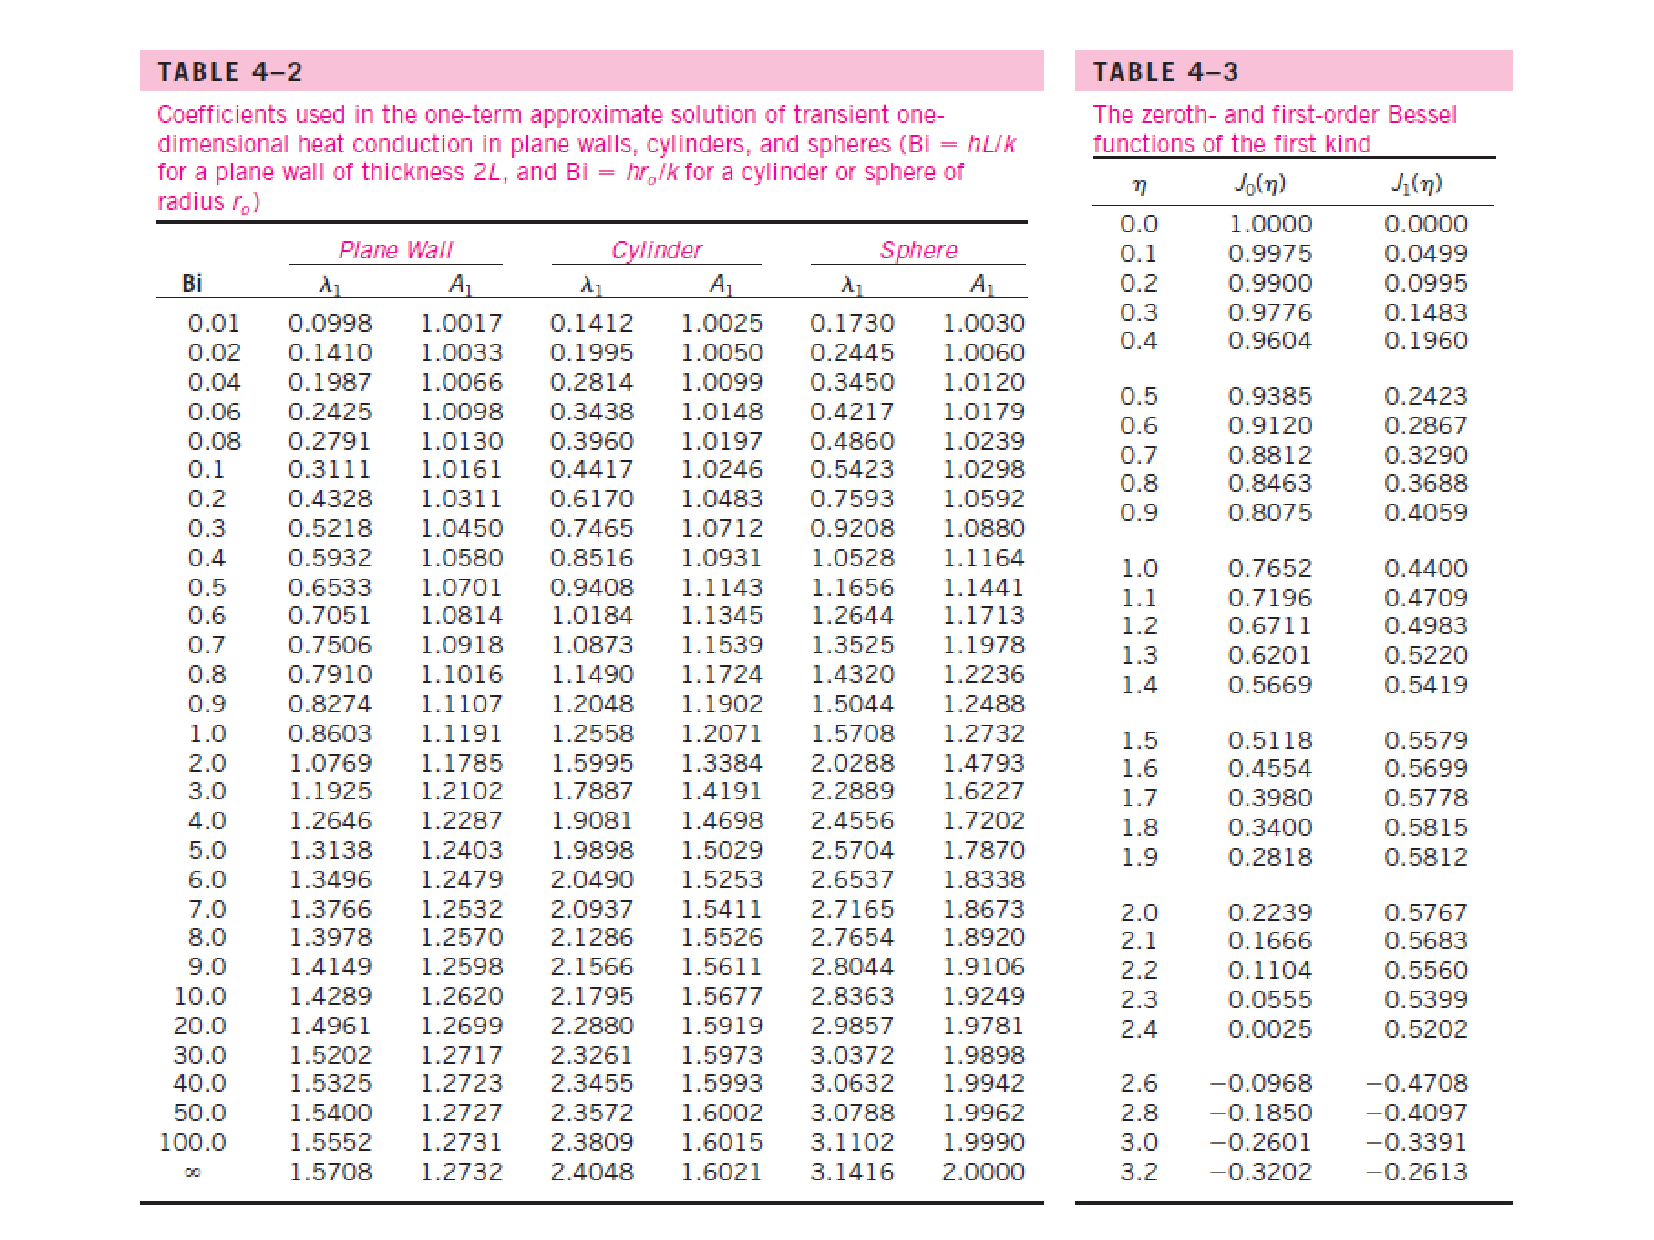
\includegraphics[width=.9\columnwidth,height=.65\columnwidth,clip]{./Pics/BaselFunctionTable}
        \end{center}
\end{frame}


\subsection{Appendix 2: Heisler and Gr\"ober Charts (extracted from [3])}\label{appendix2}
%\begin{frame}
%        \begin{center}
          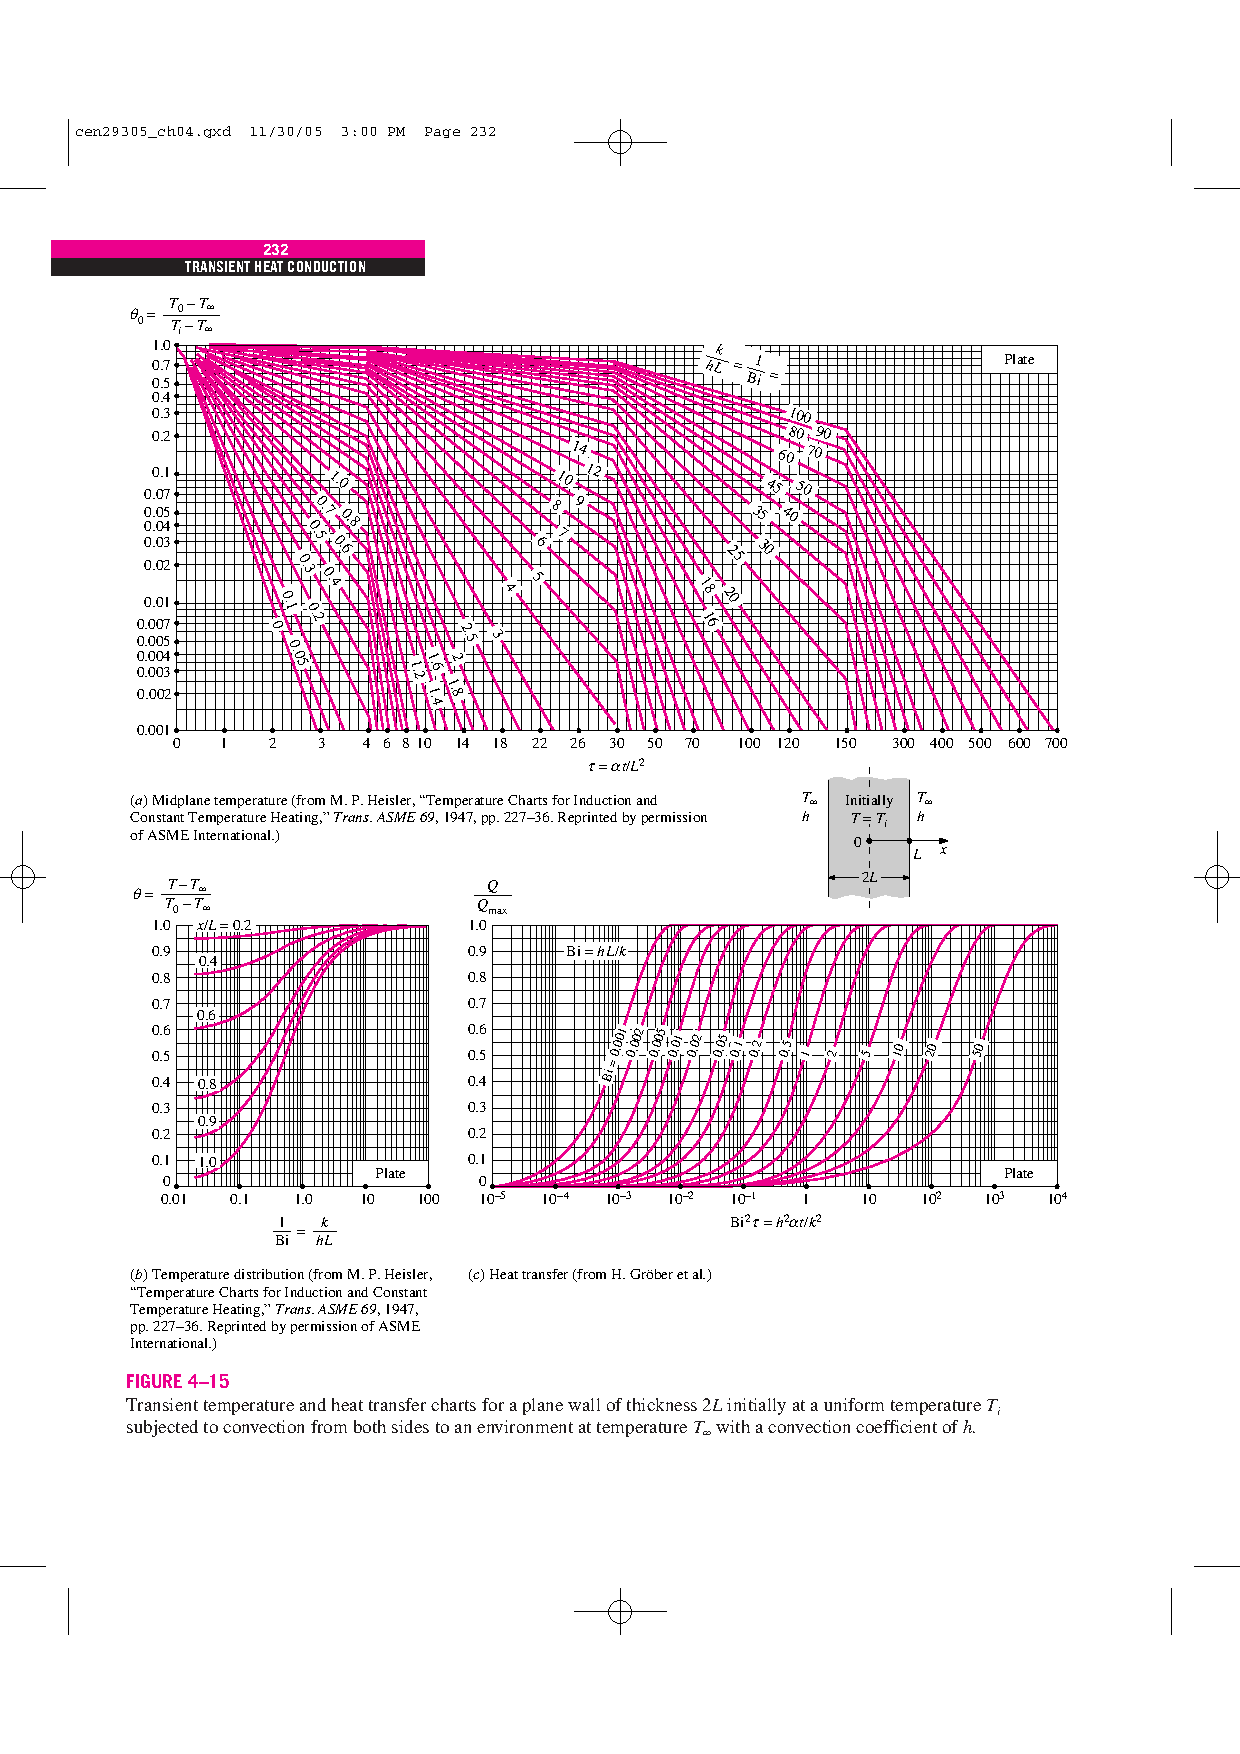
\includegraphics[width=.9\columnwidth,height=.65\columnwidth,clip]{./Pics/HeislerCharts_All}
%        \end{center}
{
  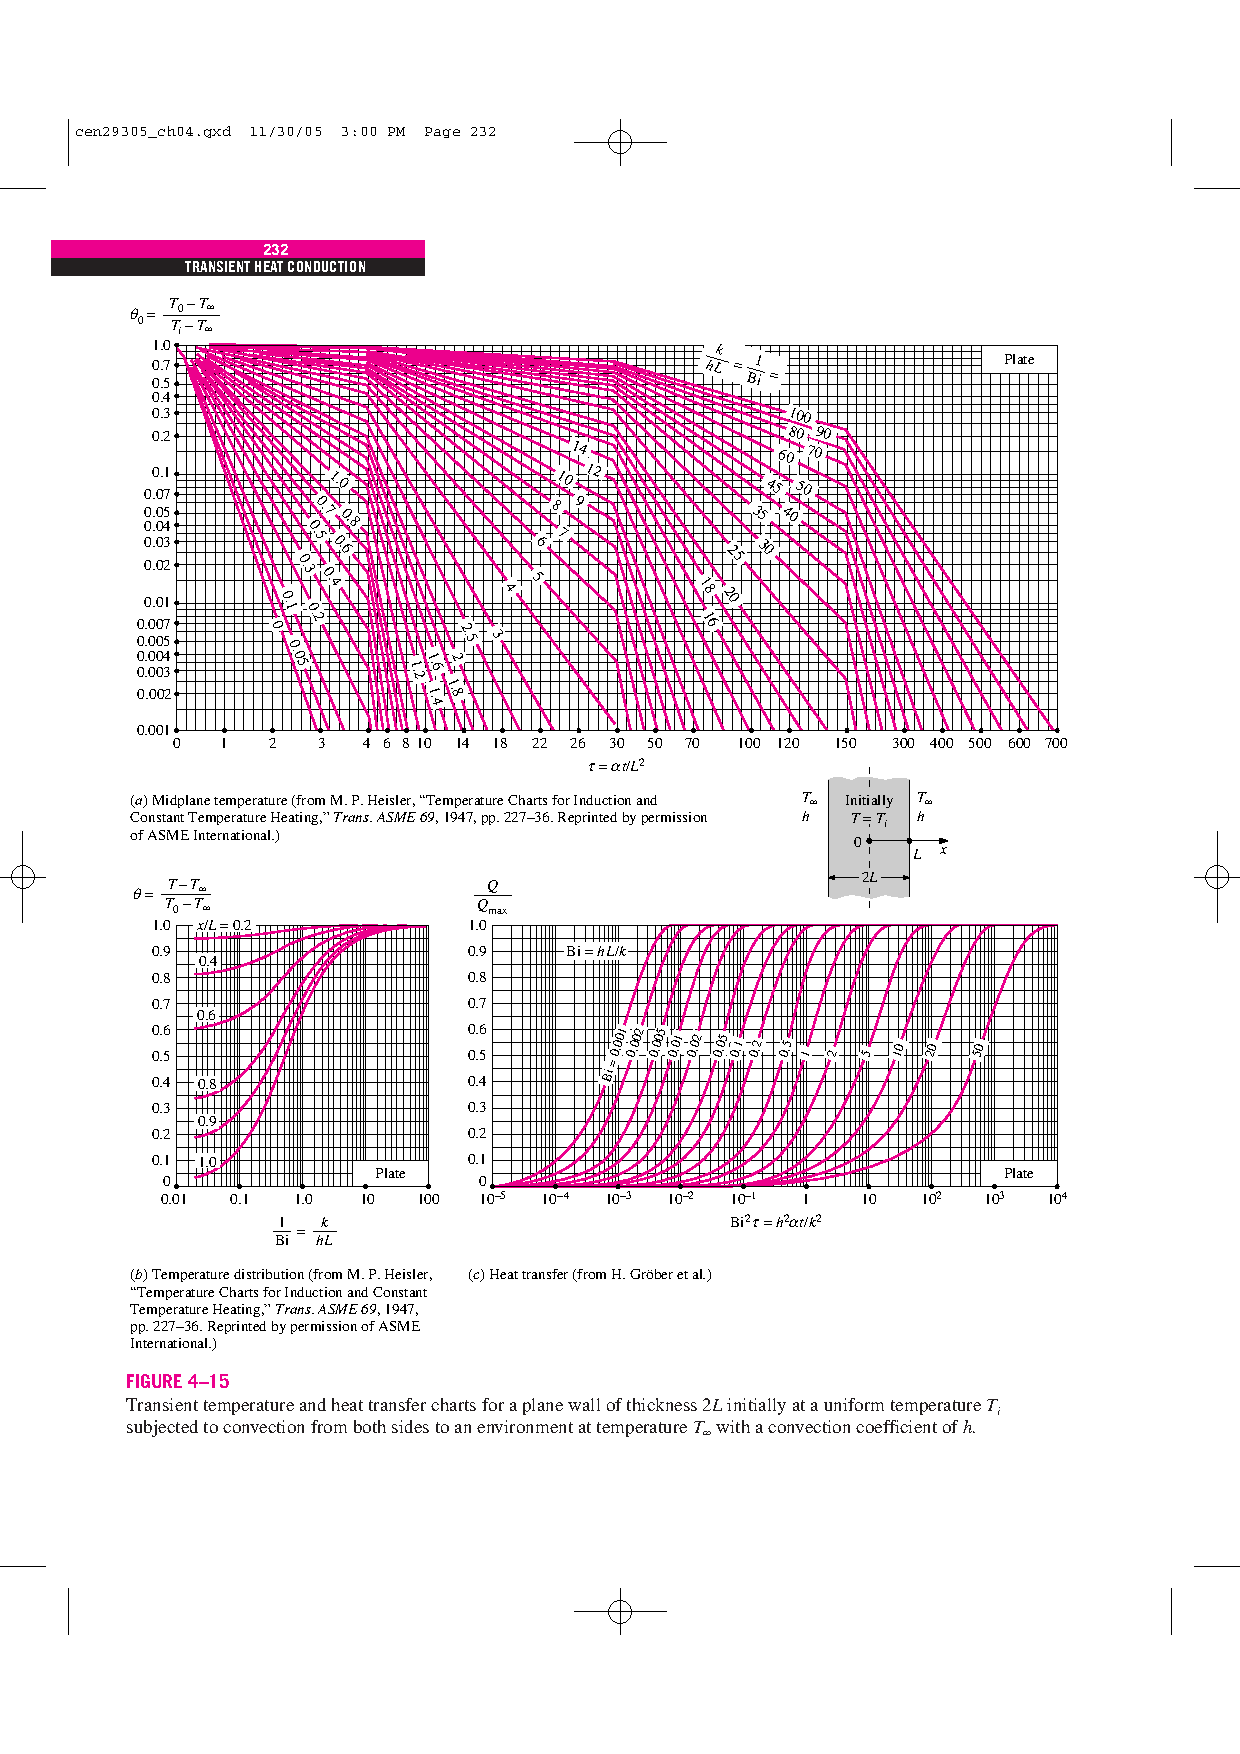
\includepdf[pages=-,fitpaper]{./Pics/HeislerCharts_All.pdf}
}
%\end{frame}


\end{document}
